\documentclass[tikz,border=5pt]{standalone}
\usepackage{pgfplots}
\pgfplotsset{compat=1.18}
\usepackage{fontspec}
\setsansfont{SourceSansPro}[
  Path = /usr/local/texlive/2024/texmf-dist/fonts/opentype/adobe/sourcesanspro/,
  UprightFont = SourceSansPro-Regular.otf,
  BoldFont = SourceSansPro-Bold.otf,
  ItalicFont = SourceSansPro-RegularIt.otf,
  BoldItalicFont = SourceSansPro-BoldIt.otf,
  Scale = 1.0
]
\usetikzlibrary{positioning}
\usepackage{xcolor}
\definecolor{primaryblue}{HTML}{012169}
\definecolor{primarygold}{HTML}{B9975B}
\definecolor{highlightyellow}{HTML}{F2A900}
\definecolor{lightbg}{HTML}{E8EDF5}
\definecolor{jet}{HTML}{1A1A1A}
\definecolor{positivegreen}{HTML}{15803D}
\definecolor{negativered}{HTML}{B91C1C}
\newcommand{\hi}[1]{{\bfseries\color{primaryblue}#1}}
\begin{document}
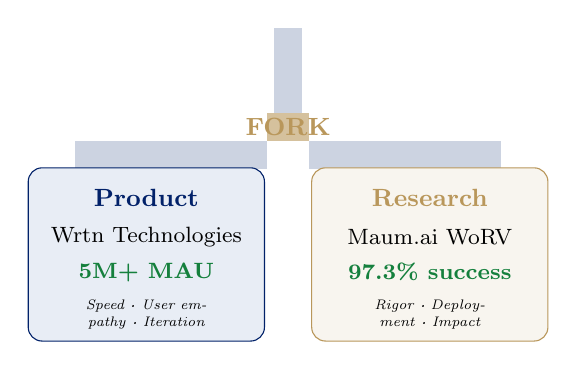
\begin{tikzpicture}[scale=0.9]
  % The single road coming in from top
  \fill[primaryblue!20] (3.3,4.8) -- (3.7,4.8) -- (3.7,3.6) -- (3.3,3.6) -- cycle;

  % Fork point
  \fill[primarygold!60] (3.2,3.6) -- (3.8,3.6) -- (3.8,3.2) -- (3.2,3.2) -- cycle;

  % Left road (Product)
  \fill[primaryblue!20] (0.5,3.2) -- (3.2,3.2) -- (3.2,2.8) -- (0.5,2.8) -- cycle;

  % Right road (Research)
  \fill[primaryblue!20] (3.8,3.2) -- (6.5,3.2) -- (6.5,2.8) -- (3.8,2.8) -- cycle;

  % Left path box
  \node[draw=primaryblue, fill=lightbg, rounded corners=5pt,
        minimum width=3.0cm, minimum height=2.2cm, align=center]
        at (1.5, 1.6) {};
  \node[font=\small\bfseries\color{primaryblue}] at (1.5, 2.4)   {Product};
  \node[font=\footnotesize, align=center]        at (1.5, 1.85)   {Wrtn Technologies};
  \node[font=\footnotesize\bfseries\color{positivegreen}, align=center]
                                                  at (1.5, 1.35) {5M+ MAU};
  \node[font=\tiny\itshape, align=center, text width=2.6cm]
                                                  at (1.5, 0.75) {Speed · User empathy · Iteration};

  % Right path box
  \node[draw=primarygold, fill=primarygold!10, rounded corners=5pt,
        minimum width=3.0cm, minimum height=2.2cm, align=center]
        at (5.5, 1.6) {};
  \node[font=\small\bfseries\color{primarygold}] at (5.5, 2.4)   {Research};
  \node[font=\footnotesize, align=center]        at (5.5, 1.85)   {Maum.ai WoRV};
  \node[font=\footnotesize\bfseries\color{positivegreen}, align=center]
                                                  at (5.5, 1.35) {97.3\% success};
  \node[font=\tiny\itshape, align=center, text width=2.6cm]
                                                  at (5.5, 0.75) {Rigor · Deployment · Impact};

  % Labels
  \node[font=\small\bfseries\color{primarygold}] at (3.5, 3.4) {FORK};
\end{tikzpicture}
\end{document}
